\begin{frame}{Das Time-Expanded Modell}
\framesubtitle{Train-Edges}
	\begin{itemize}{}
		\item Modelliere jedes "{}\textbf{Event}"{} innerhalb einer Station als eigenen Knoten. 
	\end{itemize}

	\begin{center}
		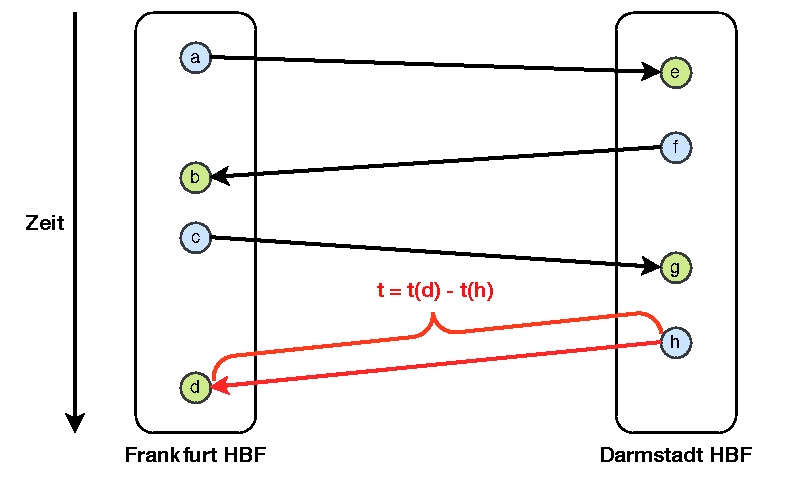
\includegraphics[width=.72\linewidth]{images/time-expanded-basic.pdf} 
	\end{center}
\end{frame}


\begin{frame}{Das Time-Expanded Modell}
\framesubtitle{Waiting-Edge}
	\begin{itemize}
		\item Erstelle eine Stationsinterne Kante, die \textbf{Exchange-Edge}. 
	\end{itemize}

	\begin{center}
	\hspace{5em}
		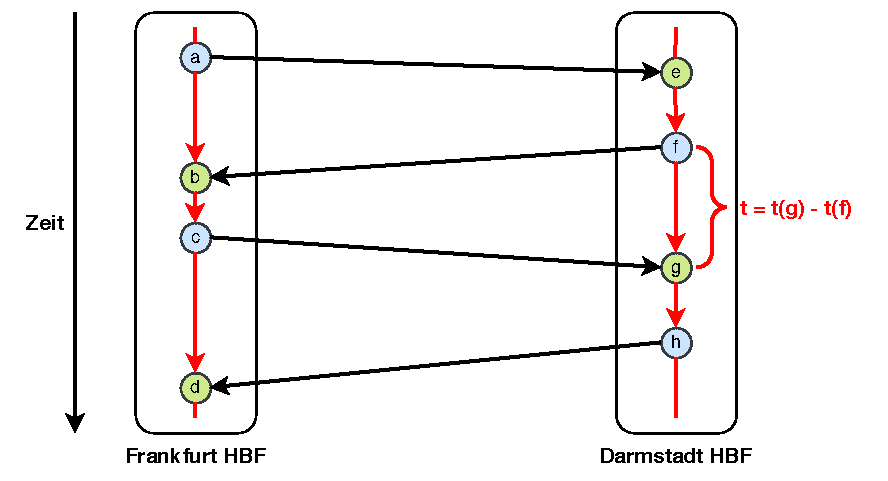
\includegraphics[width=.78\linewidth]{images/time-expanded-basic-2.pdf} 
	\end{center}
\end{frame}


\begin{frame}{Das Time-Expanded Modell}
\framesubtitle{Was bringt uns das Ganze jetzt?}
\vspace{6em}
\begin{center}
	\begin{LARGE}
		Kanten innerhalb einer Station $\approx$ "{}Umstiege"{}
	\end{LARGE}
\end{center}
\end{frame}


\begin{image-frame}
\begin{frame}{}
	\vspace{-1em}
	\begin{center}
		\begin{tikzpicture}
			\node (img1) {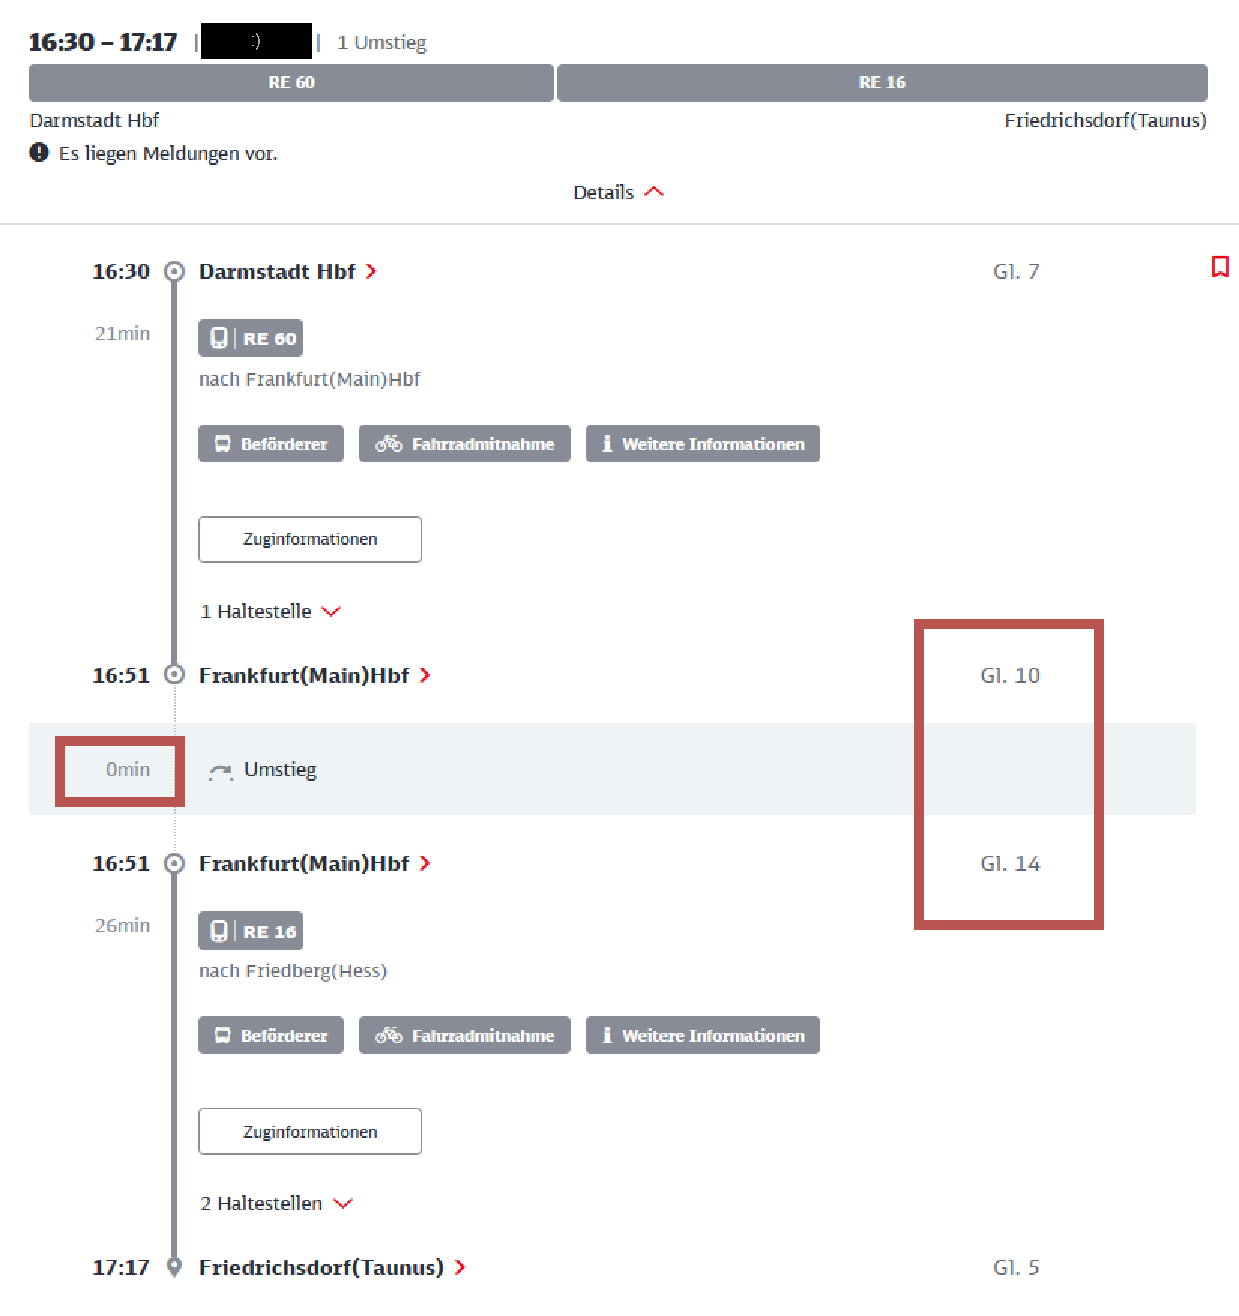
\includegraphics[width=.75\linewidth]{images/time-expanded_darmstadt-fdorf-no-interchange-time.pdf}};
			\pause
			\node (img2) at (img1.center) {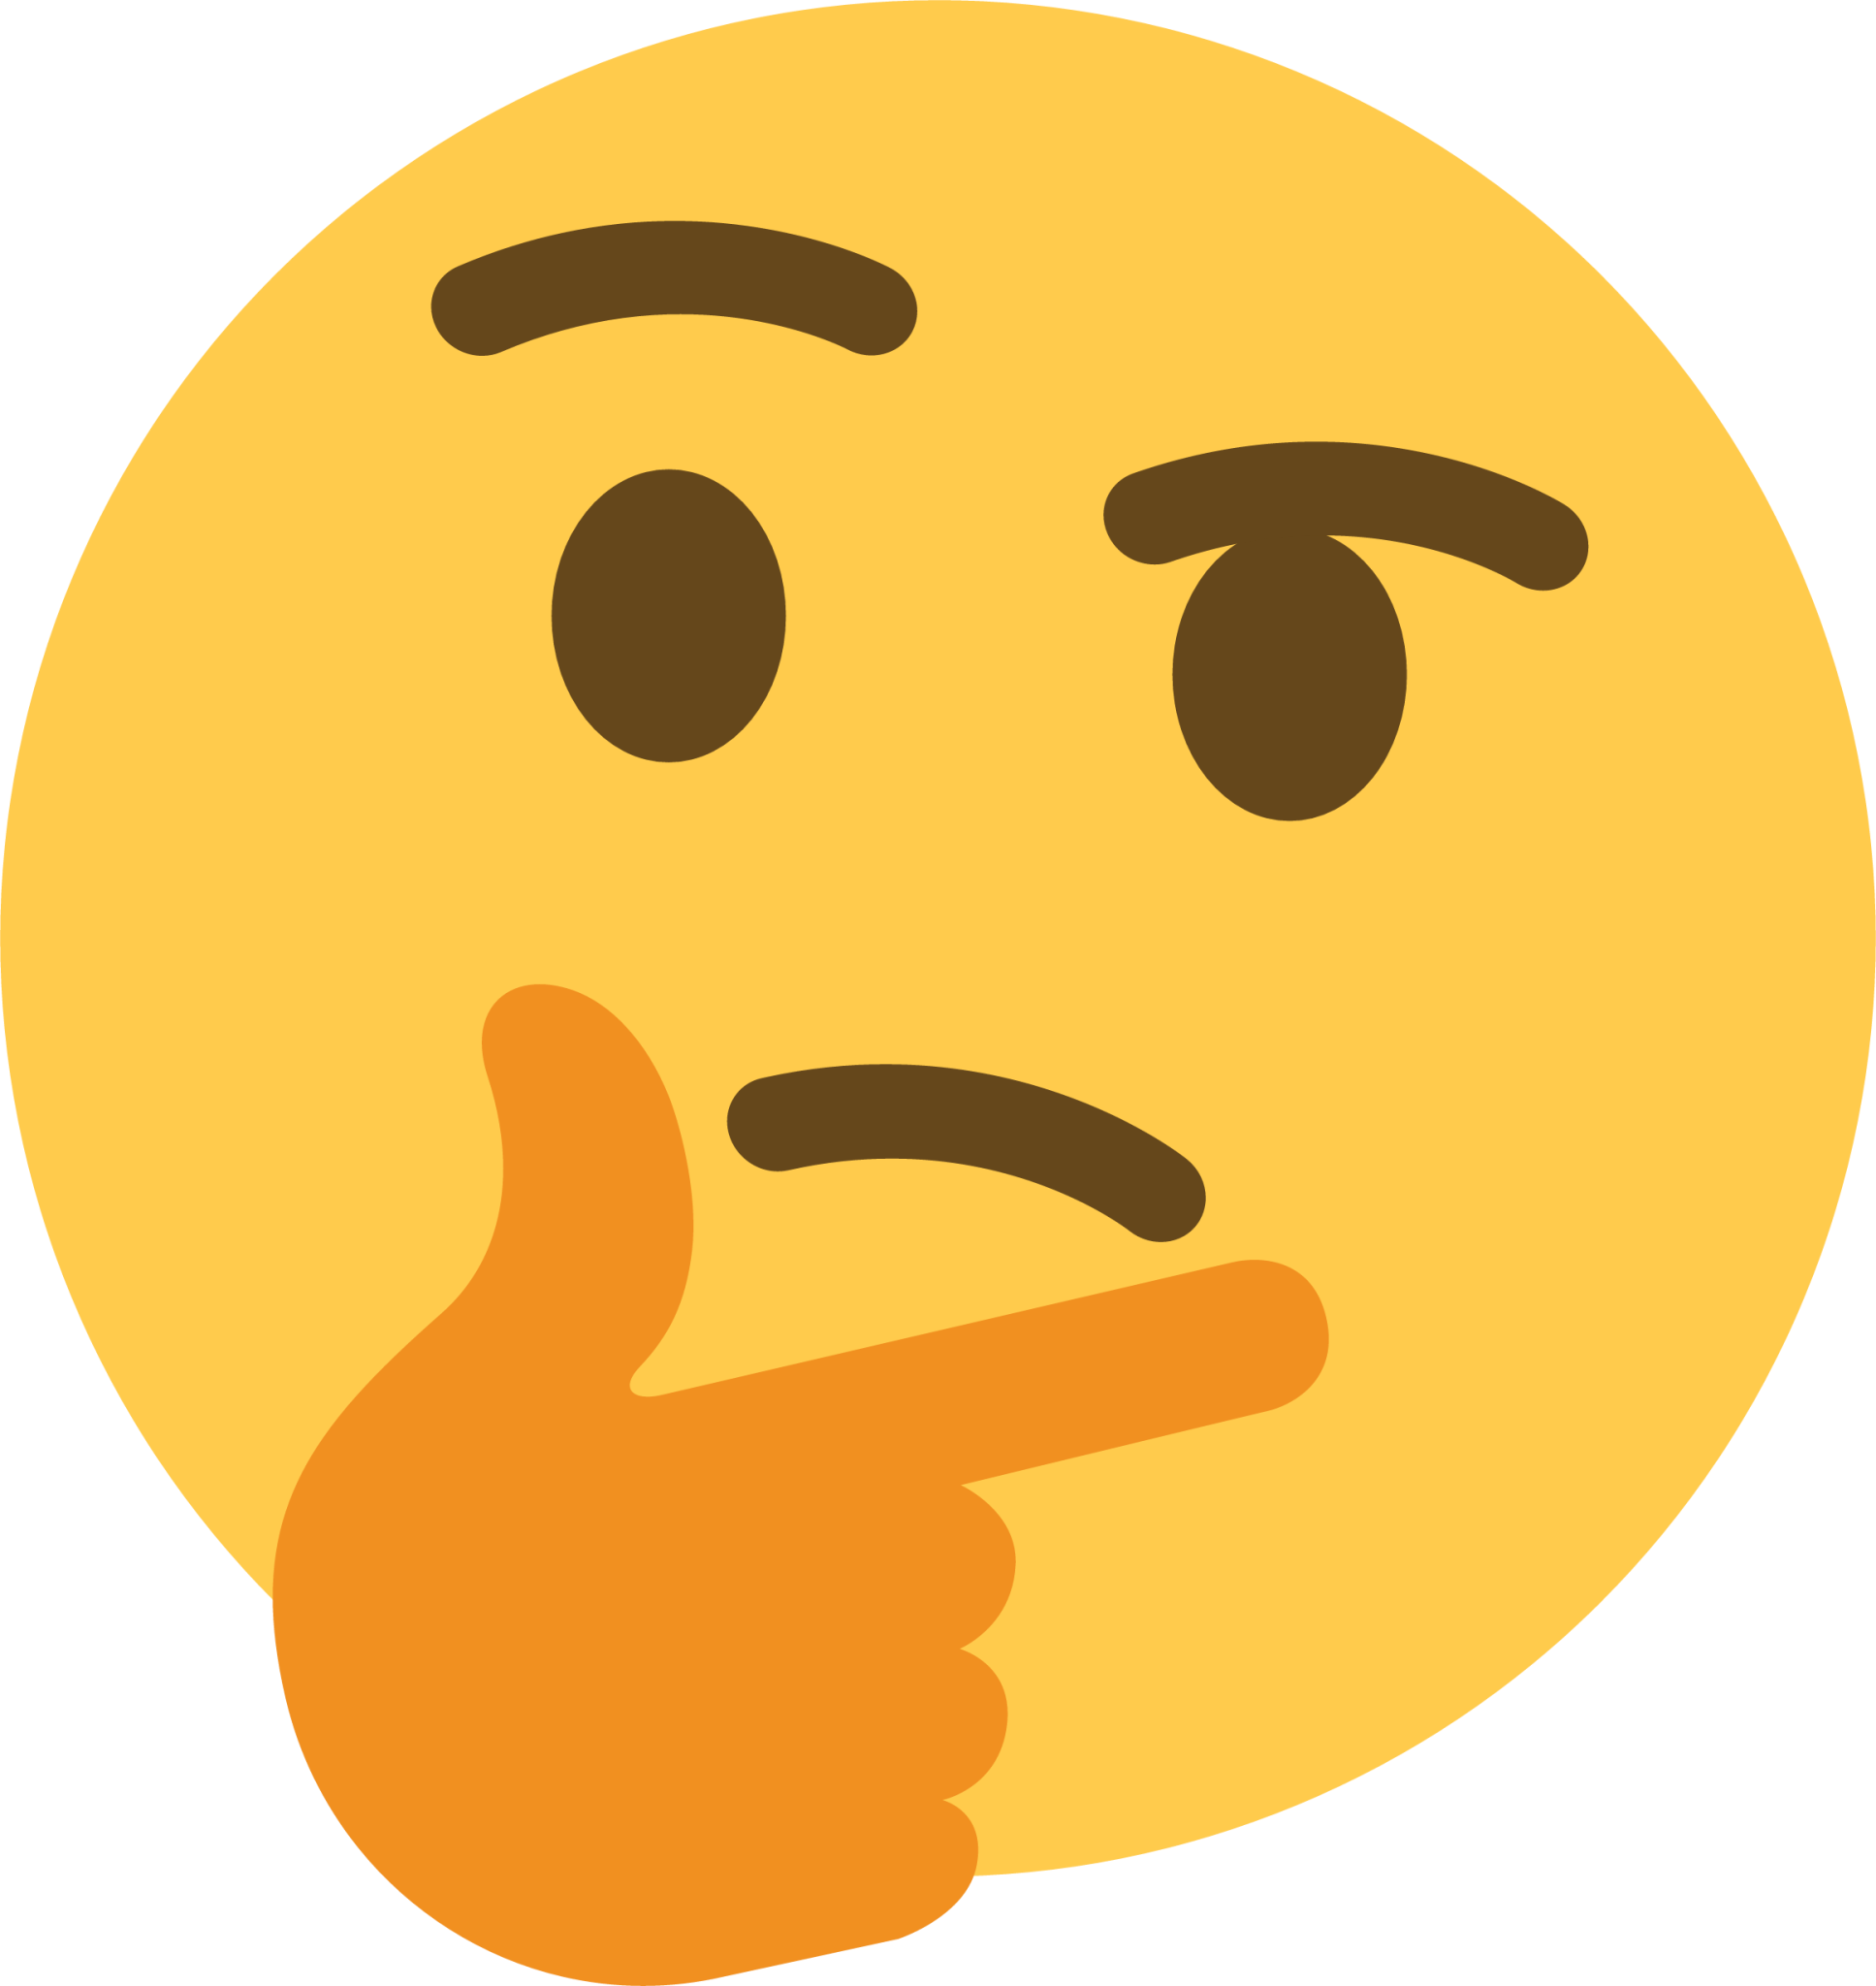
\includegraphics[height=3cm]{images/thinkingning.png}};
		\end{tikzpicture}
	\end{center}
\end{frame}
\end{image-frame}


\subsection{Umstiegszeiten}
\begin{frame}
\vspace{8em}
\begin{center}
	\begin{LARGE}
		Problem: Erhebliche Umsteigezeiten innerhalb von großen Stationen.
	\end{LARGE}
\end{center}
\end{frame}


\begin{frame}{2. Griff in die Terminologie-Kiste}
	\framesubtitle{Realistische Umstiegsregeln}
	\begin{itemize}
		\item Definiere \textcolor{brown}{Konstante} und \textcolor{purple}{Variable} Umstiegsregeln:
		\begin{enumerate}
			\item \textcolor{brown}{Standard-Umstiegszeit für alle Züge}
			\pause
			\item \textcolor{purple}{Regeln basierend auf Transferklassen \& Zuglinien}
			\pause
			\item \textcolor{purple}{Regeln zwischen einzelnen Zügen}
		\end{enumerate}
	\end{itemize}
\end{frame}


\begin{frame}{Konstante Umstiegszeiten}
	\begin{center}
		\begin{tikzpicture}
			\node (img1) {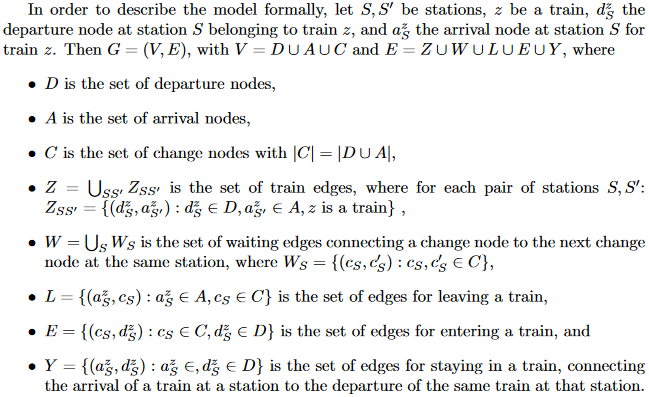
\includegraphics[height=5cm]{images/time-expanded-garble.png}};
		\end{tikzpicture}
	\end{center}
\end{frame}


\begin{frame}{Konstante Umstiegszeiten}
	\begin{itemize}
		\item Spalte Exchange-Edge in Ankunfts- und Abfahrtsknoten
	\end{itemize}

	\begin{center}
		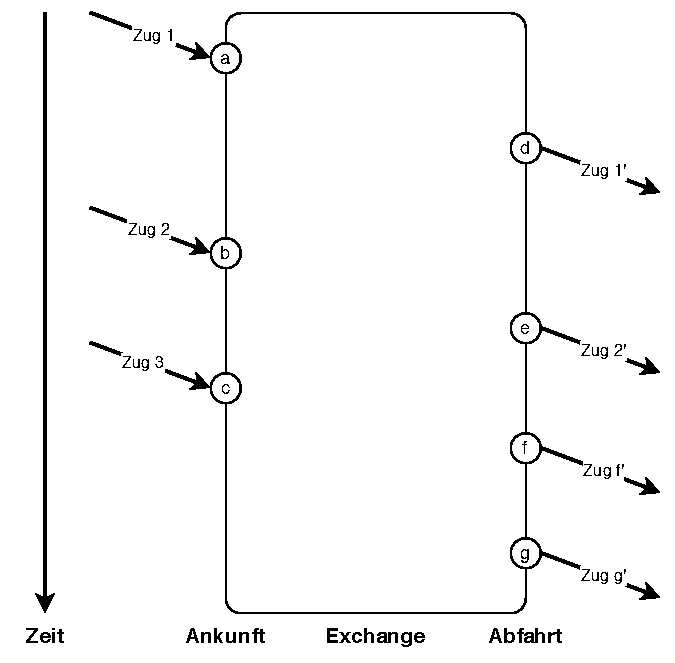
\includegraphics[height=6cm]{images/time_expanded_constant_interchange_0.pdf} 
	\end{center}
\end{frame}


\begin{frame}{Konstante Umstiegszeiten}
	\begin{itemize}
		\item Erstelle neue Exchange Edge
	\end{itemize}

	\begin{center}
		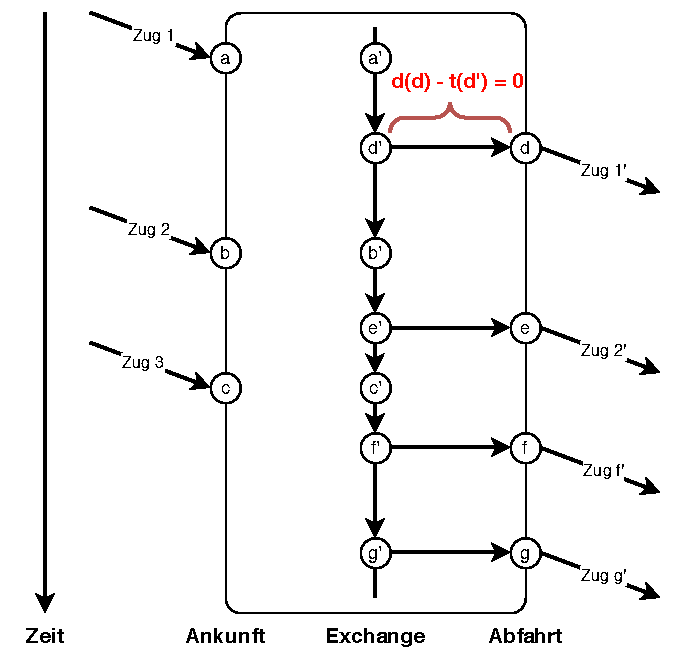
\includegraphics[height=6cm]{images/time_expanded_constant_interchange_1.pdf} 
	\end{center}
\end{frame}


\begin{frame}{Konstante Umstiegszeiten}
	\begin{itemize}
		\item Kanten von Ankunft $\rightarrow$ Exchange-Edge basierend auf min. Umstiegszeit
	\end{itemize}

	\begin{center}
		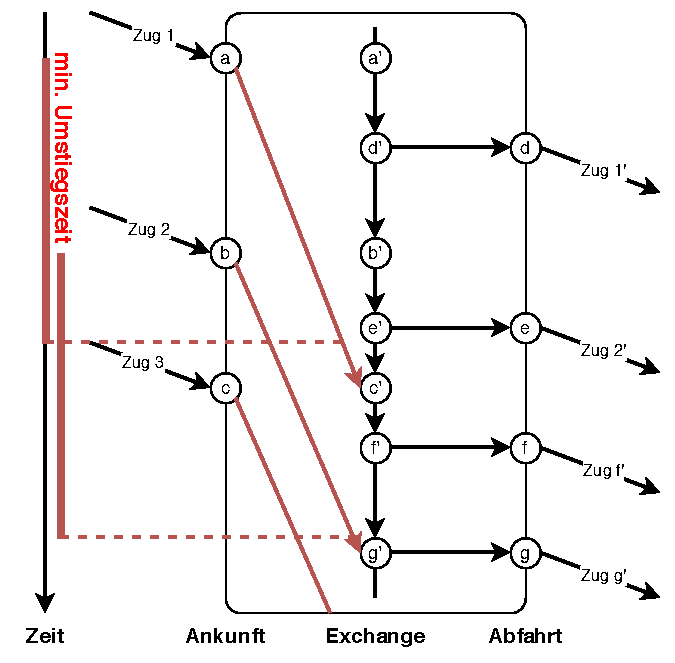
\includegraphics[height=6cm]{images/time_expanded_constant_interchange_2.pdf} 
	\end{center}
\end{frame}


\begin{frame}{Variable Umstiegszeiten}
	\begin{itemize}
		 \item Erstelle Kanten von Ankunft $\rightarrow$ Abfahrt des selben Zuges
	\end{itemize}

	\begin{center}
		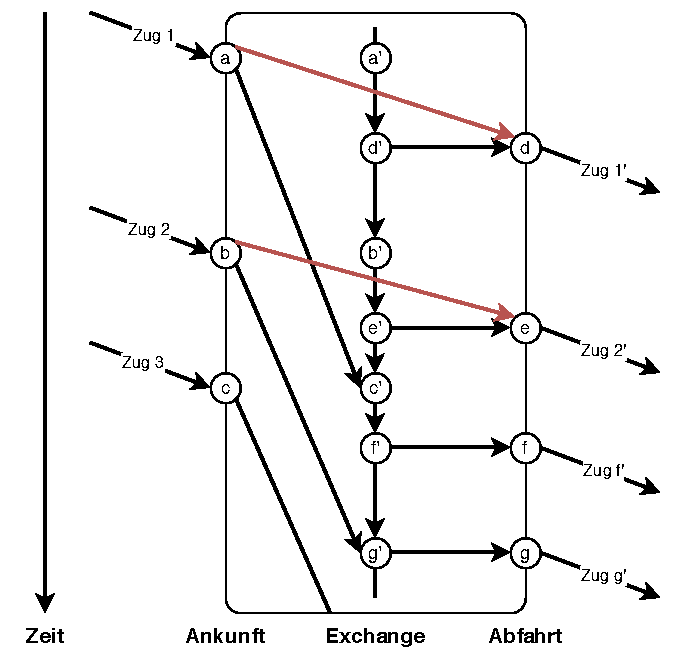
\includegraphics[height=6cm]{images/time_expanded_constant_interchange_3.pdf} 
	\end{center}
\end{frame}



\begin{frame}{Variable Umstiegszeiten}
	\begin{itemize}
		\item Weitere variable Umstiegszeiten als zzgl. Kanten
	\end{itemize}

	\begin{center}
		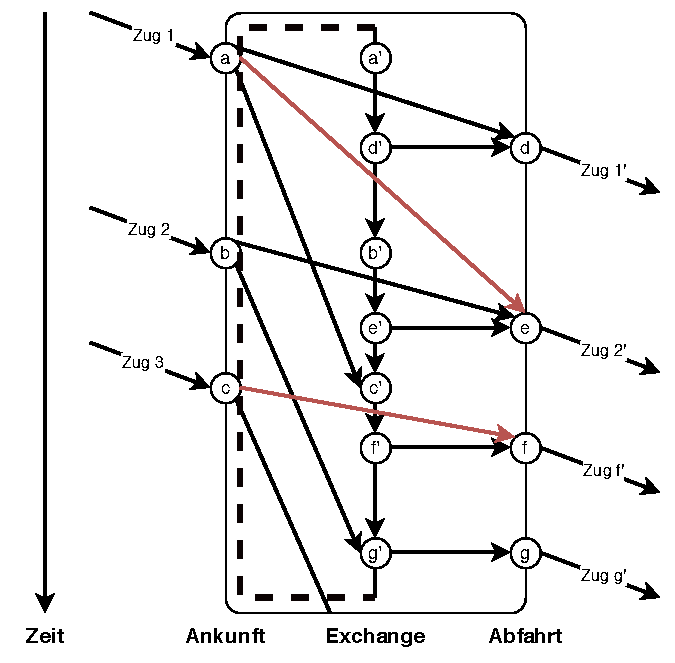
\includegraphics[height=6cm]{images/time_expanded_variable_interchange.pdf} 
	\end{center}
\end{frame}


\begin{frame}{Taktfahrplanmodellierung}
	\begin{itemize}
		\item Taktfahrplanmodellierung via Exchange-Edge-Schleife
	\end{itemize}

	\begin{center}
		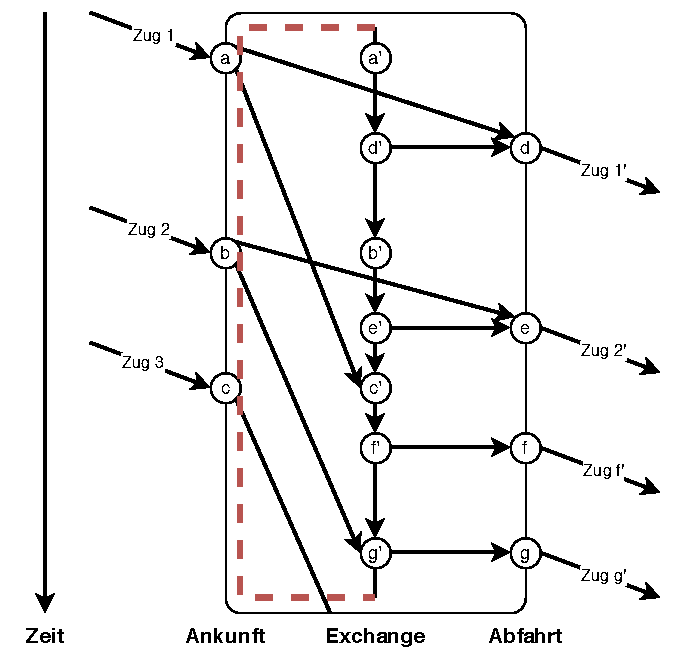
\includegraphics[height=6cm]{images/time_expanded_constant_interchange_4.pdf} 
	\end{center}
\end{frame}


\subsection{Verfeinerungen}
\begin{frame}{Verfeinerung 1: Verkehrstage}
	\begin{block}{}
		Problem: Der Takt unseres Fahrplans ist nicht nur ein Tag!
	\end{block}
	\pause
	\begin{itemize}
		\item $N$ Tage ($1440min/d$) im Taktfahrplan
		\pause
		\item Versehe Kanten mit einem Tupel aus Verkehstagen und Zeit: $\{[d], t\}$
		\item Beim SP-Durchlauf: Prüfe auf validen Tag, und bestimme Zeit für den Tag
	\end{itemize}

	\pause
	\begin{equation*}
		Tag = floor(\frac{t_{Absolut}}{1440})
	\end{equation*}

	\pause
	\begin{equation*}
		length(E) = t_{Ankunft} - t_{Abfahrt} \mod 1440
	\end{equation*}
\end{frame}


\begin{frame}{Verfeinerung 1: Verkehrstage}
	\begin{block}{}
		Problem: Wie behandeln wir besuchte Knoten beim SP-Durchlauf, die invalide sind?
	\end{block}

	\pause
	\begin{itemize}
		\item Als Beispiel am Dijkstra: 
		\begin{itemize}
			\item $dist \rightarrow \infty$
			\item Füge Knoten wieder am Ende des Sets ein ("{}Nächster"{} Tag).
		\end{itemize}
	\end{itemize}
	\vspace{5em}
	Weitere Verfeinerungen sind möglich\footnote{Pyrga et. al.: Efficient Models for Timetable Information in Public Transportation Systems}...
\end{frame}


\begin{frame}{Verfeinerung 2: Fußwege}
	\framesubtitle{Die Rückkehr der Terminologie-Kiste}
	\begin{block}{}
		Was macht Fußwege so besonders?
	\end{block}
	\pause
	\begin{itemize}
		\item Fußwege können zu jeder Zeit genutzt werden
		\item Man könnte sagen sie sind... \textit{Zeitabhängig} (Time-Dependent)...
	\end{itemize}

	\begin{center}
		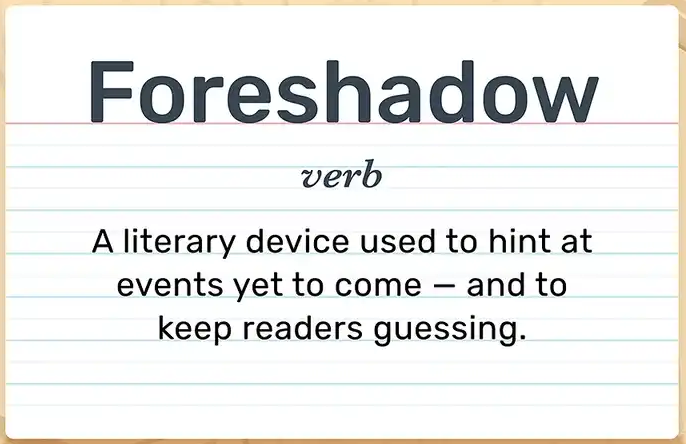
\includegraphics[height=4cm]{images/foreshadowing.png} 
	\end{center}
\end{frame}


\begin{frame}{Verfeinerung 2: Fußwege}
	\begin{itemize}
		\item Alle Fußwege im Graphen speichern ist nicht sinnvoll.
		\pause
		\item Stattdessen: Speichere Liste an Fußwegen für jede Station mit konst. Zeit
	\end{itemize}
\end{frame}


\begin{frame}{Verfeinerung 2: Fußwege}
	\begin{itemize}
		\item Nutze den Floyd-Warshall-Algorithmus
		\pause
		% Dijkstra: SP von einem Knoten zu allen anderen Knoten, nur pos. Werte
		% Bellman-Ford: SP von einem Knoten zu allen anderen Knoten, neg. Werte
		\item SP von allen Knoten zu allen anderen Knoten, negative Kantenwerte sind erlaubt
		\pause
		% Beachte Fußwege nur, wenn wir eine arrival-node verlassen
		\item Speichere Wege in jeder Station, maskiere Wege in Suchanfragen als Kanten zwischen Stationen
		% Wenn wir N stationen im Umkreis haben, und Fußwege zu den Stationen < departure_interval sind, dann ist evtl. eine Verbindung mit Fußweg als erste "Kante" die beste!
		% Starte Dijkstra mit intialer zeit != 0, der Zeit des Fussweges
		\item Beachte Fußwege als Start einer Reise!
	\end{itemize}
\end{frame}


\begin{frame}{Größenordnungen}
	\begin{itemize}
		\item Ein paar Zahlen im Jahr 2008 (\textbf{nur} Züge):
	\end{itemize}

	\begin{center}
		\begin{tabular}{ c|c } 
			Anzahl an Knoten & \\
 			\hline
 			Ankunft & 801.8 Tsd. \\
 			Abfahrt & 801.8 Tsd. \\
 			Exchange & 556.6 Tsd. \\
 			\hline
 			Gesamt & 2160.2 Tsd.
		\end{tabular}
	\end{center}
\end{frame}


\begin{frame}{Größenordnungen}
	\begin{itemize}
		\item Ein paar Zahlen im Jahr 2008 (\textbf{nur} Züge):
	\end{itemize}

	\begin{center}
		\begin{tabular}{ c|c } 
			Anzahl an Kanten & \\
 			\hline
 			Zug & 801.8 Tsd. \\
 			Weiterfahrt & 733.7 Tsd. \\
 			Ankunft & 796.7 Tsd. \\
 			Abfahrt & 796.7 Tsd. \\
 			Warten (auf Exchange-Edge) & 556.6 Tsd. \\
 			Besondere Umstiege & 20.2 Tsd. \\
 			\hline
 			Gesamtanzahl & 3704.7 Tsd.
		\end{tabular}
	\end{center}
\end{frame}



